% This file was created by tikzplotlib v0.9.1.
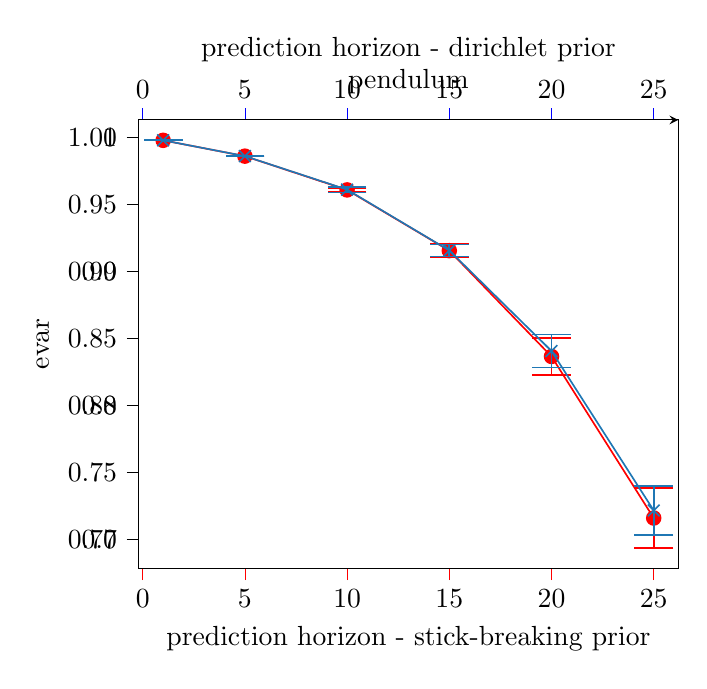
\begin{tikzpicture}

\definecolor{color0}{rgb}{0.12156862745098,0.466666666666667,0.705882352941177}

\begin{axis}[
tick align=outside,
tick pos=left,
title={pendulum},
x grid style={white!69.0196078431373!black},
xlabel={prediction horizon - stick-breaking prior},
xmin=-0.2, xmax=26.2,
xtick style={color=red},
y grid style={white!69.0196078431373!black},
ylabel={evar},
ymin=0.678587895990278, ymax=1.01282718628804,
ytick style={color=black},
ytick={0.65,0.7,0.75,0.8,0.85,0.9,0.95,1,1.05},
yticklabels={0.65,0.70,0.75,0.80,0.85,0.90,0.95,1.00,1.05}
]
\path [draw=red, semithick]
(axis cs:1,0.997587965550704)
--(axis cs:1,0.997632081285428);

\path [draw=red, semithick]
(axis cs:5,0.985482626543631)
--(axis cs:5,0.986147343944928);

\path [draw=red, semithick]
(axis cs:10,0.959034373449098)
--(axis cs:10,0.962228243837953);

\path [draw=red, semithick]
(axis cs:15,0.910126995179591)
--(axis cs:15,0.920566595399963);

\path [draw=red, semithick]
(axis cs:20,0.822797733153483)
--(axis cs:20,0.850122659860393);

\path [draw=red, semithick]
(axis cs:25,0.693780591003813)
--(axis cs:25,0.73824626074116);

\addplot [semithick, red, mark=-, mark size=7, mark options={solid}, only marks]
table {%
1 0.997587965550704
5 0.985482626543631
10 0.959034373449098
15 0.910126995179591
20 0.822797733153483
25 0.693780591003813
};
\addplot [semithick, red, mark=-, mark size=7, mark options={solid}, only marks]
table {%
1 0.997632081285428
5 0.986147343944928
10 0.962228243837953
15 0.920566595399963
20 0.850122659860393
25 0.73824626074116
};
\addplot [semithick, red, mark=*, mark size=2.5, mark options={solid}]
table {%
1 0.997610023418066
5 0.98581498524428
10 0.960631308643526
15 0.915346795289777
20 0.836460196506938
25 0.716013425872486
};
\end{axis}

\begin{axis}[
axis x line=top,
tick align=outside,
x grid style={white!69.0196078431373!black},
xlabel={prediction horizon - dirichlet prior},
xmin=-0.2, xmax=26.2,
xtick pos=right,
xtick style={color=blue},
y grid style={white!69.0196078431373!black},
ymin=0.678587895990278, ymax=1.01282718628804,
ytick pos=left,
ytick style={color=black}
]
\path [draw=color0, semithick]
(axis cs:1,0.997593341560764)
--(axis cs:1,0.997634491274506);

\path [draw=color0, semithick]
(axis cs:5,0.985494078664736)
--(axis cs:5,0.986225567410213);

\path [draw=color0, semithick]
(axis cs:10,0.958792777275507)
--(axis cs:10,0.962927500507785);

\path [draw=color0, semithick]
(axis cs:15,0.911048657378548)
--(axis cs:15,0.919942980761241);

\path [draw=color0, semithick]
(axis cs:20,0.828320283011163)
--(axis cs:20,0.852736333580737);

\path [draw=color0, semithick]
(axis cs:25,0.703333379713037)
--(axis cs:25,0.739985883789833);

\addplot [semithick, color0, mark=-, mark size=7, mark options={solid}, only marks]
table {%
1 0.997593341560764
5 0.985494078664736
10 0.958792777275507
15 0.911048657378548
20 0.828320283011163
25 0.703333379713037
};
\addplot [semithick, color0, mark=-, mark size=7, mark options={solid}, only marks]
table {%
1 0.997634491274506
5 0.986225567410213
10 0.962927500507785
15 0.919942980761241
20 0.852736333580737
25 0.739985883789833
};
\addplot [semithick, color0, mark=x, mark size=3, mark options={solid}]
table {%
1 0.997613916417635
5 0.985859823037475
10 0.960860138891646
15 0.915495819069894
20 0.84052830829595
25 0.721659631751435
};
\end{axis}

\end{tikzpicture}
